% 
% Lecture Template for ME3050 -  Dynamics Modeling and Controls - Tennessee Technological University
%
% Spring 2020 - Summer 2020
% Tristan Hill, May 07, 2020
% Dyanmics Review - Topic 2 - Coordinate Systems
%

%\documentclass{beamer}                         % for presentation (has nav buttons at bottom)
\documentclass[handout]{beamer}  % for handout 
\usepackage{beamerthemesplit}
\usepackage{amsmath}
\usepackage{listings}
\usepackage{multicol}
\usepackage{framed}

\beamertemplateballitem

\definecolor{TTUpurple}{rgb}{0.3098, 0.1607, 0.5176} % TTU Purple (primary)
\definecolor{TTUgold}{rgb}{1.0000, 0.8666, 0.0000} % TTU Gold (primary)

\setbeamercolor{palette primary}{bg=TTUpurple,fg=TTUgold}
\setbeamercolor{palette secondary}{bg=black,fg=TTUgold}
\setbeamercolor{palette tertiary}{bg=black,fg=TTUpurple}
\setbeamercolor{palette quaternary}{bg=TTUgold,fg=black}
\setbeamercolor{structure}{fg=TTUpurple} % itemize, enumerate, etc
\setbeamercolor{section in toc}{fg=TTUpurple} % TOC sections

%\usefonttheme{professionalfonts}

\newcommand{\Lagr}{\mathcal{L}} % lagrangian

\newcommand{\vspccc}{\vspace{6mm}\\} % large vertical space
\newcommand{\vspcc}{\vspace{4mm}\\}   % medium vertical space
\newcommand{\vspc}{\vspace{2mm}\\}     % small vertical space

\newcommand{\hspcccc}{\hspace{10mm}} % large horizontal space
\newcommand{\hspccc}{\hspace{6mm}} % large horizontal space
\newcommand{\hspcc}{\hspace{4mm}}   % medium horizontal space
\newcommand{\hspc}{\hspace{2mm}}     % small horizontal space


\author{ME3050 - Dynamics Modeling and Controls}%\\Tennessee Technological University \\} % original formatting from Mike Renfro, September 21, 2004

\newcommand{\MNUM}{2\hspace{2mm}} % Module number
\newcommand{\TNUM}{2\hspace{2mm}} % Topic number 
\newcommand{\moduletitle}{Dynamics Review }
\newcommand{\topictitle}{Coordinate Systems } 

\title{Module \MNUM - \moduletitle}

\date{May 29, 2020}

\begin{document}

\lstset{language=MATLAB,basicstyle=\ttfamily\small,showstringspaces=false}

\frame{\titlepage \center\begin{framed}\Large \textbf{Topic \TNUM - \topictitle}\end{framed} \vspace{5mm}}

% Section 0: Outline

\frame{

\large \textbf{Topic \TNUM - \topictitle} \vspace{3mm}\\

\begin{itemize}
	\item Using Different Coordinate Systems\vspace{3mm}\\ % Section 1
	\item Cartesian\vspace{3mm}\\% Section 2
	\item Polar and Cylindrical\vspace{3mm}\\ %Section 3
	\item Spherical \vspace{3mm}\\  %Section 4
	\item Others ? \vspace{3mm}\\  %Section 5
\end{itemize}
}

% Section 1:
\section{Using Different Coordinate Systems}

\frame{
\frametitle{Using Different Coordinate Systems}

It is often convienent to use different coordinate systems as a reference for different types of problems. \vspc

You, the engineer and designer must choose the coordinate system.

}

% Section 2: 
\section{Cartesian}

\frame{
\frametitle{Cartesian}

The \href{https://en.wikipedia.org/wiki/Cartesian_coordinate_system}{Cartesian Coordinate System} 


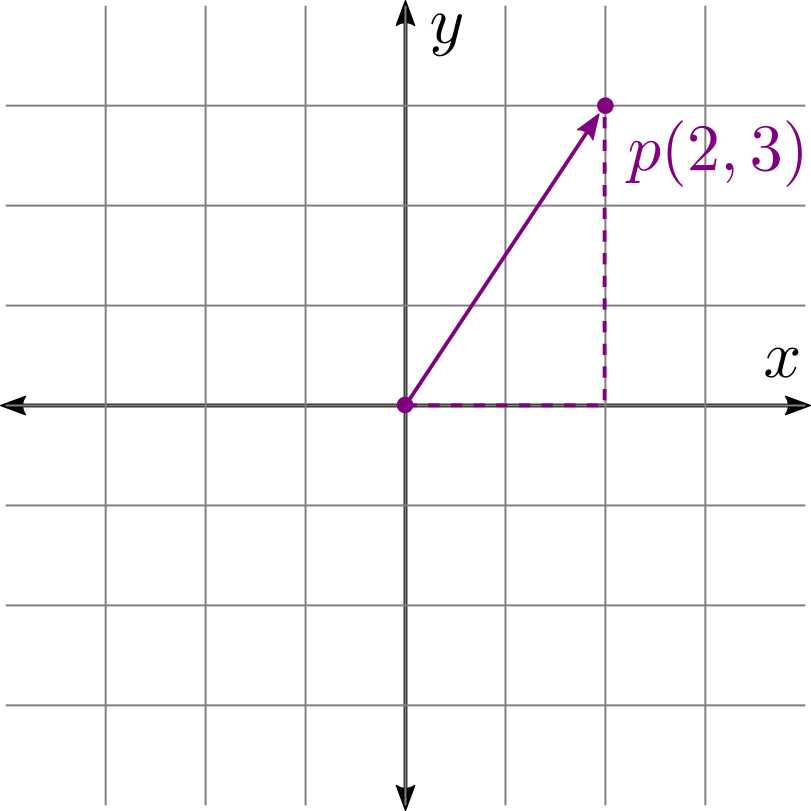
\includegraphics[scale=.175]{cartesian.png} \hspccc \hspccc
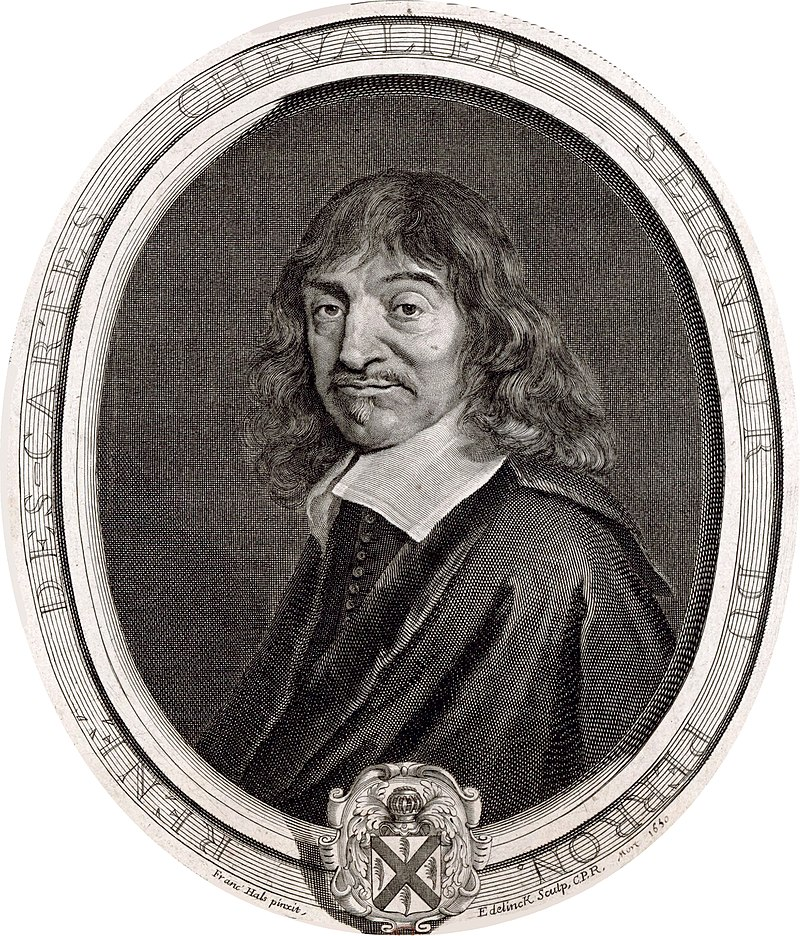
\includegraphics[scale=.125]{Descartes.jpg} \\ \hspace{80mm} {\tiny \href{https://en.wikipedia.org/wiki/Ren\%C3\%A9_Descartes}{Image: Wikipedia} }

}

\frame{
\frametitle{Rotated Cartesian}

It is common to use a Cartesian coordinate system that has been rotated such that it is aligned with a particular problem. 

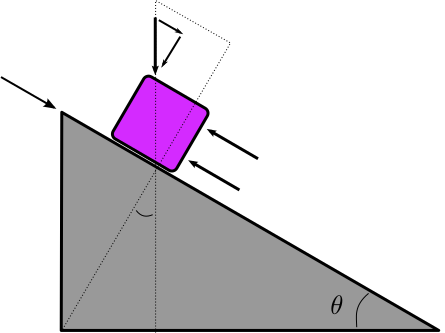
\includegraphics[scale=.4]{sliding_block.png}

}


% Section 3: 
\section{Polar and Cylindrical}

\frame{
\frametitle{Polar and Cylindrical}

For problems involving rotation it is convient to use polar or cylindrical coordinate systems. Conversion from Cartesian to polar  is straightforward using trigonometry. 

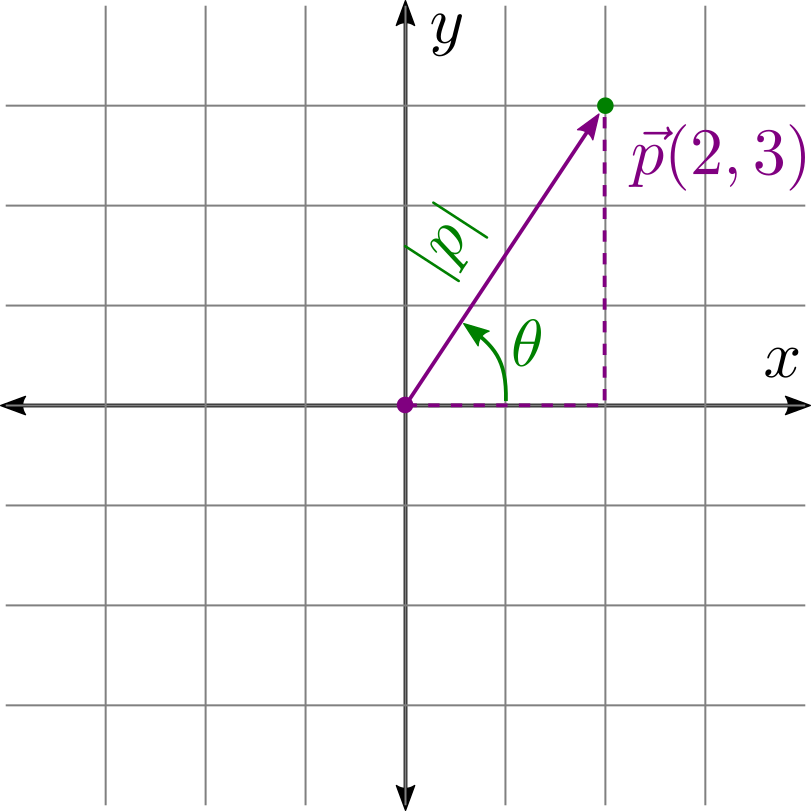
\includegraphics[scale=.18]{polar.png} \hspccc \hspccc 
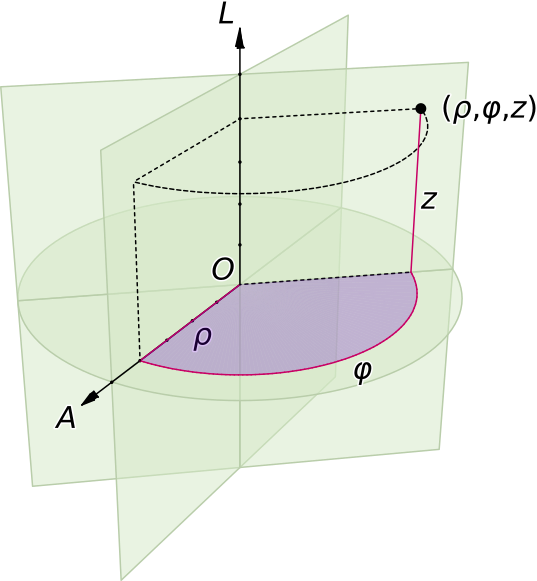
\includegraphics[scale=.275]{cylindrical.png}\\ \hspace{80mm} {\tiny \href{https://en.wikipedia.org/wiki/Cylindrical_coordinate_system}{Image: Wikipedia} }

}

% Section 4:
\section{Spherical}

\frame{
\frametitle{Spherical}

``The spherical coordinate system generalizes the two-dimensional polar coordinate system...'' {\tiny \href{https://en.wikipedia.org/wiki/Spherical_coordinate_system}{Wikipedia} }

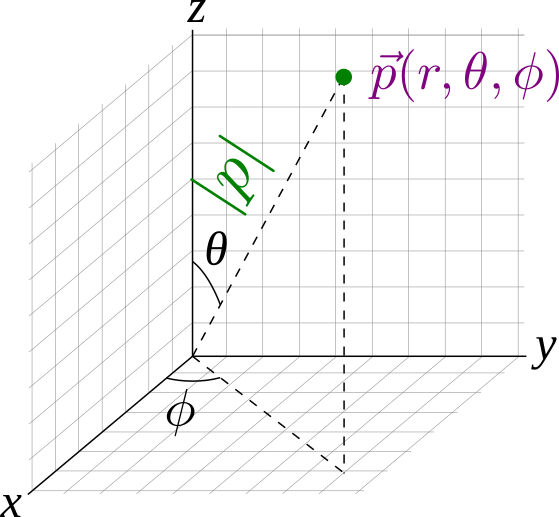
\includegraphics[scale=.3]{spherical_fig1.png} \hspccc \hspccc
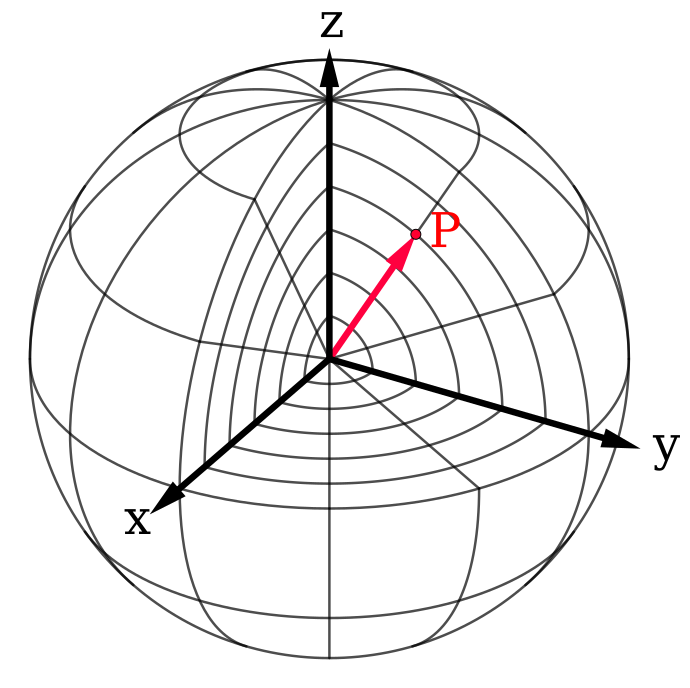
\includegraphics[scale=.2]{spherical_fig2.png}  \\ {\tiny \href{https://en.wikipedia.org/wiki/Spherical_coordinate_system}{Image: Wikipedia} } \hspace{60mm} {\tiny \href{https://en.wikipedia.org/wiki/Spherical_coordinate_system}{Image: Wikipedia} }


}

% Section 5:
\section{Others ?}

\frame{
\frametitle{Others ?}

Do you know of any other systems that are used?

}
	
\end{document}



